\begin{frame}{Slave Motor (Right)}
	\framesubtitle{Setpoint and Response}
  \begin{itemize}
		\item Feeds the metal strip $\Rightarrow$ Lower velocity
		\item Dynamic Model: $RM(s) \simeq \frac{7.128}{6.0665s+1}$
	\end{itemize}
			\centering
				\includegraphics[width=.9\textheight]{RM_systemID.png}
\end{frame}

\begin{frame}{Slave Motor}
  \framesubtitle{Controller Design}
  \begin{block}{P Controller}
	\begin{itemize}
		\item Fast response, better tracking than PI
		\item Steady state error rejection not necessary due to cascade control
	\end{itemize}
  \end{block}
\end{frame}

\begin{frame}{Slave Motor}
\framesubtitle{Tuning Result}
\centering
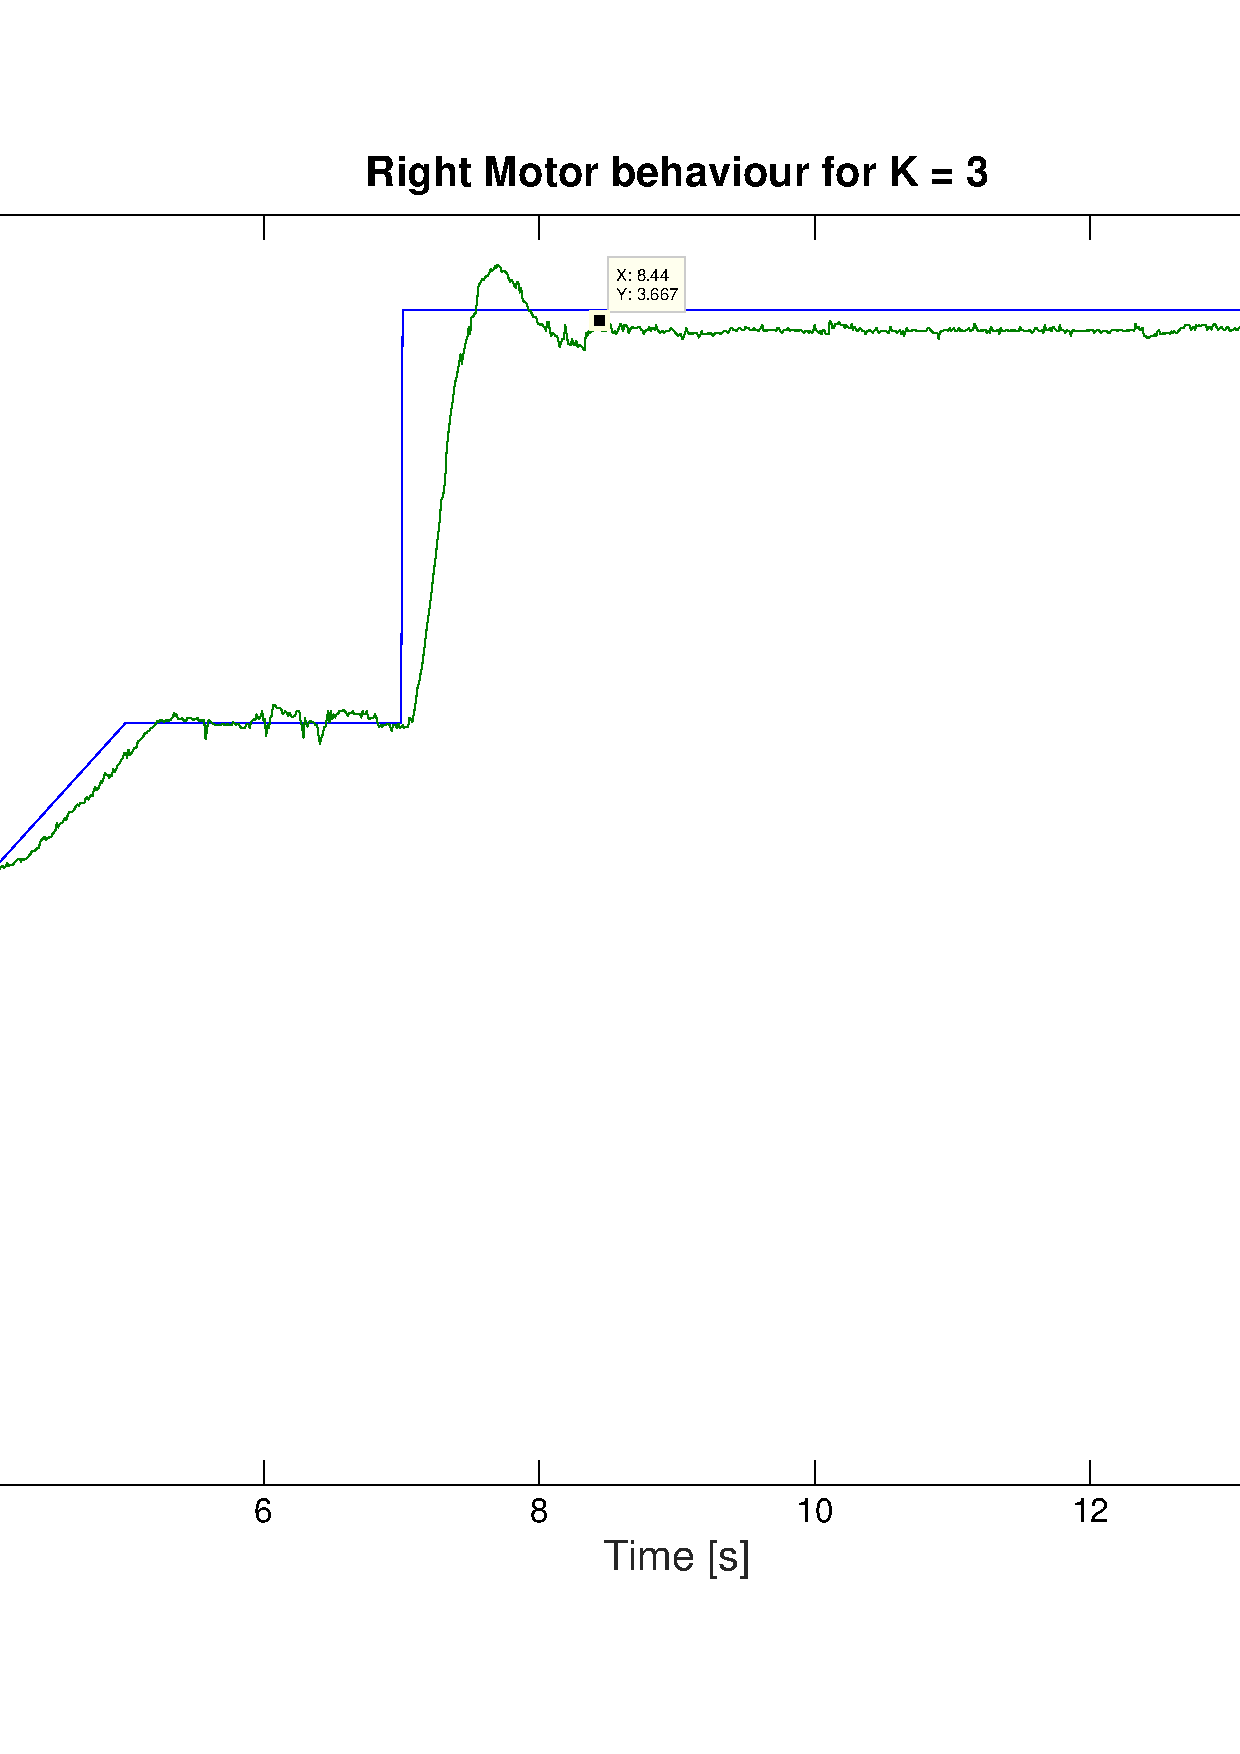
\includegraphics[width = \textwidth]{RM_K3.pdf}
\end{frame}

\begin{frame}{Slave Motor}
\framesubtitle{Conclusion}
\begin{block}{Final tuning}
\begin{itemize}
\item P Controller for fast tracking
\item Gain $K_P = 3$ to avoid actuator saturation
\item Overshoot is due to non linearities and higher order effects
\end{itemize}
\end{block}
\begin{block}{Closed loop experimental response}
\[Slave(s) \simeq \frac{0.9577}{0.2428s + 1}\]
\end{block}
\end{frame}
